\documentclass[12pt, a4paper, openany]{report}
\def\VersionRapport{1.0}
\usepackage[utf8]{inputenc} % un package
\usepackage[T1]{fontenc}      % un second package
\usepackage[francais]{babel}  % un troisième package
\usepackage{layout}
\usepackage[top=2.7cm, bottom=2.5cm, left=3.5cm, right=3cm]{geometry}
\usepackage{setspace}
\frenchbsetup{StandardLists=true} % à inclure si on utilise \usepackage[french]{babel}
%\usepackage{enumitem}
\usepackage[shortlabels]{enumitem}
\usepackage{amssymb}
\usepackage{color}
\usepackage{listings}
\definecolor{dkgreen}{rgb}{0,0.6,0}
\definecolor{gray}{rgb}{0.5,0.5,0.5}
\definecolor{mauve}{rgb}{0.58,0,0.82}
\definecolor{rougecerise}{rgb}{0.73,0.043,0.043}
\lstset{frame=tb,
  language=Matlab,
  aboveskip=3mm,
  belowskip=3mm,
  showstringspaces=false,
  columns=flexible,
  basicstyle={\small\ttfamily},
  keywordstyle=\color{blue},
  commentstyle=\color{dkgreen},
  stringstyle=\color{mauve},
  breaklines=true,
  breakatwhitespace=true,
  tabsize=3,
  breaklines=true,
  morekeywords={matlab2tikz},
  morekeywords=[2]{1}, 
  keywordstyle=[2]{\color{black}},
  identifierstyle=\color{black},
  numbers=left,
  numberstyle={\tiny \color{black}},
  numbersep=9pt, 
  emph=[1]{for,end,break},
  emphstyle=[1]\color{red}
}
\usepackage{multirow} % pour les tableaux
\usepackage[table]{xcolor} % pour les tableaux
\usepackage{verbatim}
%\usepackage{subcaption}
\usepackage{graphicx}
\usepackage{moreverb}
\usepackage{url}
\usepackage{pst-all}
\usepackage{eso-pic,graphicx}
\usepackage{caption} 
\usepackage[colorlinks=true,urlcolor=blue,linkcolor=red]{hyperref}
\usepackage{array}
\usepackage[toc,page]{appendix}
\usepackage[off]{auto-pst-pdf}
\usepackage{hyperref} % pour le sommaire table des matières
\AddThinSpaceBeforeFootnotes % à insérer si on utilise \usepackage[french]{babel}
\FrenchFootnotes % à insérer si on utilise \usepackage[french]{babel}
\usepackage{fancyhdr}
\pagestyle{headings}
\usepackage{pifont}  %pour les puces
\usepackage{amsmath} %pour les puces
\usepackage{subfig}
\usepackage{verbatim} % pour le code en annexe 
%%%%%%%colones 
\newcolumntype{R}[1]{>{\raggedleft\arraybackslash }b{#1}}
\newcolumntype{L}[1]{>{\raggedright\arraybackslash }b{#1}}
\newcolumntype{C}[1]{>{\centering\arraybackslash }b{#1}}
%%%%%%% 
\renewcommand{\appendixpagename}{Annexes}
\renewcommand{\appendixtocname}{Annexes}
\title{Theme: Compte Rendu SLI 1}
\author{TEVENINO \bsc{Namataiki} \\ KHERBICHE \bsc{Ali}}
\date{2018-2019}
%new
\newcommand{\HRule}{\rule{\linewidth}{0.5mm}}

\begin{document}

%\selectlanguage{francais}
\pagenumbering{arabic} 
\makeatletter
\begin{titlepage}
\begin{sffamily}
\begin{center}
    % Upper part of the page. The '~' is needed because \\
    % only works if a paragraph has started.
    
\includegraphics[scale=0.5]{Logo_UT3.jpg}~\\[1cm]
    \textsc{\LARGE M1 ISTR-RODECO  }\\[1cm]
    \textsc{\Large Compte Rendu SLI 2}\\[1cm]
    % Title
    \HRule \\[0.4cm] % saut de ligne
    { \huge  \textsc {Etude simulée de la commande par retour de sortie d'un système de bacs d'eau \\[0.4cm] }}

    \HRule \\[1cm]   % sous de ligne 
    
\includegraphics[scale=0.1]{logomaster.jpg}
    \\[1cm]
    % Author and supervisor
    \begin{minipage}{0.4\textwidth}
      \begin{flushleft} \large
         \textsc{\emph {Fait par:} \\KHERBICHE Ali\\ TEVENINO Namataiki}  
          \newline
          Promotion 2018-2019 \\
      \end{flushleft}
    \end{minipage}
    \begin{minipage}{0.4\textwidth}
      \begin{flushright} \large
        %%\emph{Tuteur et}
        \emph{Tuteurs:} \textsc{M.Frédéric GOUAISBAUT\\M.Sylvain DUROLA}
      \end{flushright}
    \end{minipage}
    \vfill
    % Bottom of the page
    {\large Décembre 2018}
  \end{center}
  \end{sffamily}                
  \end{titlepage}  
\makeatother
   
%*********************** somaire **************
\renewcommand{\contentsname}{Sommaire}
\tableofcontents
%*********************** listes des figures **************
\listoffigures
%*********************** listes des tableaux **************
%\listoftables

 \chapter*{\textsc {Introduction}}
	\chaptermark{\textsc {Introduction}}

	\section{\textsc {Manipulation du TP}}
	
\paragraph{}	 
Le but de de cette manipulation est de réaliser un asservissement de niveau par retour de sortie. En effet, le vecteur d'état du procédé hydraulique n'est pas entièrement accessible par la mesure. On se propose ainsi de mettre en oeuvre l'estimation de l'état par un observateur.

\section{ \textsc{Présentation du système}}
\paragraph{}
Dans ce TP, nous utilisons le même procédé que celui utilisé dans le TP du module I4 intitulé "Modélisation, analyse et commande d'une distribution hydraulique à trois bacs d'eau". Voici, ci-dessous, les caractéristiques essentielles de la manipulation. On considère ici le procédé trois bacs :

\begin{figure}
\centering
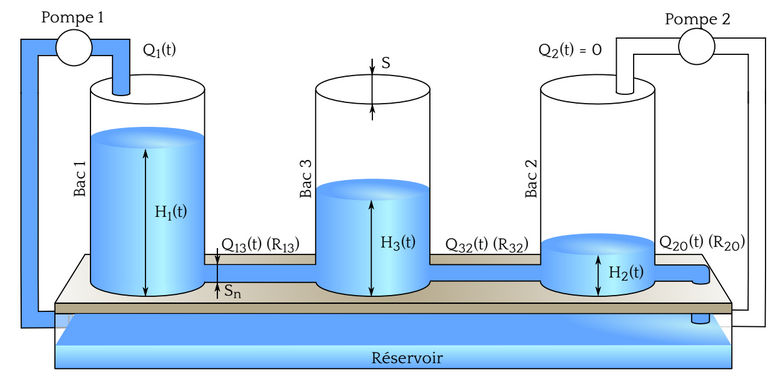
\includegraphics[scale = 0.5]{bac-deau.png}
\caption{Procédé trois bacs}
\label{fig11}
\end{figure}
 
 \paragraph{} La figure 1 représente le système du TP. Il est composé de trois bacs cylindriques en plexiglas de section S. Ces trois bacs sont disposés en série (de gauche à droite, on trouve les bacs 1, 3 et 2) et sont reliés par des tuyaux d'écoulement de section $S_n$.
\paragraph{} Le dernier bac 2 se vide par un cylindre, également de section $S_n$, dans le réservoir situé sous les trois bacs. Deux pompes de débit $Q_1(t)$ et $Q_2(t)$ permettent de remplir respectivement les bacs 1 et 3 avec l'eau récupérée dans le réservoir. Le système fonctionne donc ici en circuit fermé. 
\paragraph{} Les valeurs données par le constructeur sont $S=0,0154m^2$ et $S_n=5,10^{-5}m^2$. Les pompes obéissent à la relation $V_{qi}(t)=kQ_i(t)+b$, $i=1,2$. Avec $k=1,6.10^5$ et $b=-9.2592$. Où $V_{qi}(t)$ et $Q_i(t)$ représentent respectivement la tension appliquée à la pompe i et le débit correspondant.
\paragraph{} Les pompes sont alimentées par une tension comprise entre [-10V;10V]. Ainsi ke débit maximal, $Q_{max}$ délivré par une pompe est de $12.10^{-5}m^3/s$ lorsque la tension appliquée est de +10V. Les capteurs de niveau d'eau sont supposés linéaires autour du point de fonctionnement. Leur caractéristique est modélisé par l'équation $H_i(t)=k_iV_{h_i}(t)+b_i$, où $H_i$ est exprimé en mètres.

\section{\textsc{Le modèle linéarisé}}

\paragraph{} Nous considérons le procédé actionné par la seule pompe n1. Son débit $Q_1$ est compris entre [0,$Q_{max}$] suivant sa tension d'alimentation; le débit $Q_2$ délivré par la pompe 2 sera nul tout au long de la manipulation. Ainsi, les différentes hauteurs $H_1(t)$, $H_2(t)$ et $H_3(t)$ respectent par conséquent la condition $H_1(t)\ge H_3(t)\ge H_2(t)$. La seule mesure disponible lors de cette manipulation est la mesure de la hauteur d'eau $H_1(t)$.
\paragraph{} Le travail sera effectué sur un modèle aux faibles variations autou d'un point d'équilibre $H_0$ et un débit $Q_{10}$ à ce point d'équilibre de telle sorte que :\\

\begin{equation*}
\left\lbrace
\begin{array}{ccc}
Q_1(t) = q_1(t)+Q_{10} \\
H_1(t) = h_1(t)+H_{10}. \\
H_3(t) = h_3(t)+H_{30}. \\
H_2(t) = h_2(t)+H_{20}
\end{array}\right.
\end{equation*}
 
Avec $H_0 = [H_{10}~~H_{20}~~H_{30}]^T$ et $Q_{10}=3,5.10^{-5}$.\\

Les variations de hauteurs $h_1$, $h_2$ et $h_3$  vérifient la condition suivante :
$$h_1(t) \ge h_3(t) \ge h_2(t)$$.\\

En rappelant que la sortie mesurée est la hauteur d'eau $H_1(t)$, ce qui permet d'obtenir la variation de hauteur d'eau $h_1(t)$. Le modèle d'état linéarisé autour du point d'équilibre du procédé est donné par :

\begin{figure}
\centering
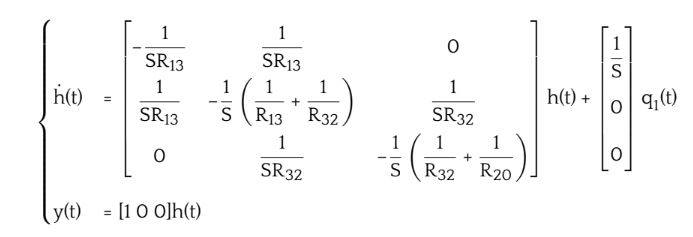
\includegraphics[scale = 0.5]{modele_detat_linearise.jpg}
\label{fig12}
\end{figure}

\paragraph{} Avec $h(t)=[h_1(t)~~h_2(t)~~h_3(t)]$. De manière conventionnelle, les matrices dynamique de commande et d'observation seront notées A, B et C. 
\paragraph{} On rappelle que $R_{ij}$ représente la résistance à l'écoulement dans les tuyaux reliant les bacs i et j :\large
$$R_{ij}=\frac{2\sqrt{|H_{i0}-H_{j0}|}}{a_{ij}}$$\normalsize
\paragraph{} Avec les trois coefficients d'écoulement : $a_{13}=0,4753S_n\sqrt{2g}$, $a_{32}=0,4833S_n\sqrt{2g}$ et $a_{20}=0,9142S_n\sqrt{2g}$.


 \chapter{\textsc {Analyse et calcul d'une loi de commande par retour d'état} }
 %\chaptermark{\textsc {Analyse et calcul d'une loi de commande par retour d'état}}
 
	\section{\textsc {Commandabilité du modèle linéarisé}} 
 	
 	\paragraph{}
 		Calcul de la matrice de commandabilité $Co=\begin{bmatrix} B&BA&A^{2}B \end{bmatrix} $:
 		
 		\begin{center}
			
			$Co$=$\begin{bmatrix}
			64.9351&-0.5975&0.0110\\
			0&0.5975&-0.0173\\
			0&0&0.0064
			\end{bmatrix}$	
			 			
		\end{center} 		 
		
		La matrice de commandabilité est triangulaire supérieure ce qui fait que son rang vaut 3 car il n'éxiste aucune relation linéaire entre ses colonnes ou entre ses lignes.\\
		\textbf{Conclusion:} Le modèle linéarisé est bien commandable vu que le rang de la matrice $Co$ est égale au nombre de valeurs propres que possède la matrice dynamique $A$. 
		
		\section{\textsc {La loi de commande par retour d'état}} 
		
		\begin{center}
		%\includegraphics[scale=0.4]{bobb.png} 
		\captionof{figure}{\textit Schéma SIMULINK du système en boucle fermée avec retour d'état}
		\label{fig1}
		\end{center}
		
		\paragraph{}
			Afin de calculer les paramètres du retour d'état soit le gain matriciel $K$ et le pré-compensateur $N$ nous devons choisir des valeurs pour les pôles désirés $P_{des}=\begin{pmatrix} P_1 & P_2 & P_3 \end{pmatrix} $ qui respectent les spécificités du cahier des charges.\\
		
		\paragraph{} Du cours de SLI2 on trouve que le temps de réponse $t_r =\frac{3}{|Re(vp)|} $ avec $vp$ : valeur propre et vu qu'une spécificité dit que $t_r \leqslant 90s$ alors on trouve:\\
		
		\begin{center}
				
				$t_r =\frac{3}{|Re(vp)|}\leqslant 90 $\\[1cm]
				$\Rightarrow|Re(vp)| \geqslant \frac{3}{90} \simeq 0.033 $\\[1cm]
				$\Rightarrow Re(vp) \geqslant 0.033 \wedge Re(vp) \leqslant -0.033$
		\end{center}
		Si $\Rightarrow Re(vp) \geqslant 0.033$ alors notre système est instable, donc la plus lente valeur propre autrement appelée mode dominant doit être inférieur ou égal à $-0.033$.\\\\
		Nous choisissons alors les valeurs désirés suivantes $P_{des}=\begin{bmatrix} -0.033&-0.15&-0.12 \end{bmatrix} $
\chapter{\textsc {Implémentation de la loi de commande} }
 \chaptermark{\textsc {Implémentation de la loi de commande}}

	\section{\textsc {Calcul d'un observateur minimal identité}} 
	 \subsection{\textsc {Observabilité du modèle linéarisé}} 
	 
	 \paragraph{}
 		Calcul de la matrice d'observabilité $OBSV=\begin{bmatrix} C\\CA\\CA^{2} \end{bmatrix} $:
 		
 		\begin{center}
			
			$OBSV$=$\begin{bmatrix}
			1&0&0\\
			-0.0092&0.0092&0\\
			0.00017&-0.00027&0.001
			\end{bmatrix}$	
					 			
		\end{center} 		
				
		La matrice d'observabilité est triangulaire inférieure ce qui fait que son rang vaut 3 car il n'éxiste aucune relation linéaire entre ses colonnes ou entre ses lignes,\label{OBSV} \hyperref[Annexe D]{voir Annexe D.}\\
		
		\textbf{Conclusion:} Le modèle linéarisé est bien observable vu que le rang de la matrice $OBSV$ est égale au nombre de valeurs propres que possède la matrice $(PI_d-A)$. 
		
	 \subsection{\textsc {Calcul de l'observateur minimal identité}}
	 
	 \paragraph{} Le but de cet observateur est de recontsruire les états non mesurables\\
	  $\widehat{h}(t)=\begin{bmatrix} \widehat{h_2}\\ \widehat{h_3} \end{bmatrix}$ tel que: $\widehat{h_2}\rightarrow h_2$ et $\widehat{h_3}\rightarrow h_3$.\\ 
	 
	 Du cours de SLI2 on a:
	 
	 \begin{center}
	 $\dot s(t)= F s(t) +(FG-GA_{11}+A_{21})y(t)+(B_2-GB_1)u(t)$\\[0.25cm]
	 $\widehat{x}(t)=s(t)+Gy(t)$\\[0.25cm]
	 Ici: $\widehat{x}(t)=\widehat{h}(t) \quad y(t)=h_1(t) \quad u(t)=q_1(t)$
	 \end{center}
	 	
	Avec:

		\begin{center}
			
			$A_{11}= -0.009202 \quad A_{12}=\begin{bmatrix} 0.009202&0 \end{bmatrix} \quad A_{21}=\begin{bmatrix} 0.009202\\0 \end{bmatrix} \quad A_{22}= \begin{bmatrix} -0.019831 & 0.010629\\0.010629 & -0.048646 \end{bmatrix} $\\[0.5cm]
			$B_1=64.93506 \quad B_2=\begin{bmatrix} 0\\0 \end{bmatrix}$\\[0.25cm]
			$G= \begin{bmatrix} g_1\\g_2 \end{bmatrix}$\\[0.25cm]
			$F=A_{22}-GC$\\[0.25cm]
			$\tilde{G}= FG-GA_{11}+A_{21}$\\[0.25cm]
			$\tilde{H}= B_2-GB_1$
			
		\end{center}
		
		\paragraph{} Comme pour calculer le gain $K$, les valeurs du gain $G$ et celles de la nouvelle matrice dynamique $F$ vont être calculées en respectant l'équivalence: $ \Psi(F)= \Psi(P_{des})$ ou $ \Psi(A_{22}-GC)= \Psi(P_{des})$. N'oublions pas que l'observateur admet un temps de réponse 5 fois plus rapide que celui du système bouclé par retour d'état alors: $ P{des} = \begin{bmatrix} 5P_2&5P_3 \end{bmatrix}$. \label{calobs} \hyperref[Annexe E]{Voir Annexe E}, on trouve:
		
		\begin{center}
		
			$G= \begin{bmatrix} 139.30\\3954.60 \end{bmatrix} \quad F=A_{22}-GC= \begin{bmatrix} -1.301670&0.010629\\-36.379600&-0.048646 \end{bmatrix}$	\\[0.25cm]
			$\tilde{G}= \begin{bmatrix} -138\\-5223.66 \end{bmatrix} \quad \tilde{H}= \begin{bmatrix} -9.0455 \times 10^{3} \\ -2.5679 \times 10^{5} \end{bmatrix}  $
		
		\end{center}
		
		A la fin nous aurons: 
		
		\begin{center}
	 $\dot s(t)= \begin{bmatrix} -1.301670&0.010629\\-36.379600&-0.048646 \end{bmatrix} s(t) + \begin{bmatrix} -138\\-5223.66 \end{bmatrix} h_1(t)+ \begin{bmatrix} -9.0455 \times 10^{3} \\ -2.5679 \times 10^{5} \end{bmatrix} q_1(t)$\\[0.25cm]
	 $\widehat{h}(t)=s(t)+ \begin{bmatrix} 139.30\\ 3954.60 \end{bmatrix} h_1(t)$\\[0.25cm]
	 \end{center}
	 
	 \begin{center}
		%\includegraphics[scale=0.4]{bobb.png} 
		\captionof{figure}{\textit Schéma bloc SIMULINK avec observateur}
		\label{fig4}
		\end{center}
\chapter*{\textsc {Conclusion}}
	\chaptermark{\textsc {Conclusion}}
	
	\paragraph{}
	Cette séance de travaux pratique très théorique a renforncé nos connaissances en SLI2 vues en cours et en travaux dirigés, à la fin de la séance nous avons pu acquérir le savoir de calculer un observateur sous MATLAB, le construire et enfin le simuler sous SIMULINK. Cette manipulation jouera beaucoup sur l'évolution de nos révisions pour l'examen final.   
\begin{appendices}

\chapter*{Annexe A}
	\addcontentsline{toc}{chapter}{Annexe A}		
	
	Code MATLAB qui calcule la matrice de commandabilité,\label{Annexe A} \hyperref[Co]{Retour vers section 1.1}
	
	\begin{lstlisting}	
S=0.0154;
Sn=5*10^-5;
g=9.81;
H10=0.27474;
H20=0.0299;
H30=0.1368;
H00=0;
a13=0.4753*Sn*sqrt(2*g);
a32=0.4833*Sn*sqrt(2*g);
a20=0.9142*Sn*sqrt(2*g);

R13=(2*sqrt(H10-H30))/a13;
R32=(2*sqrt(H30-H20))/a32;
R20=(2*sqrt(H20-H00))/a20;

A=[-1/(S*R13) 1/(S*R13) 0;
    1/(S*R13) -(1/S)*((1/R13)+(1/R32)) 1/(S*R32);
    0 1/(S*R32) -(1/S)*((1/R32)+(1/R20))]
B=[ 1/S; 0; 0]
C=[1 0 0];
D=[0];

sys=ss(A,B,C,D);

Co=ctrb(sys);
rang_co=rank(Co);
	\end{lstlisting}

\end{appendices}


\chapter*{Annexe B}
	\addcontentsline{toc}{chapter}{Annexe B}		
	
	Code MATLAB qui calcule le gain matriciel K,\label{Annexe B} \hyperref[K]{Retour vers section 1.2}
	
	\begin{lstlisting}	
P2=[-0.12 -0.15];
P=[-0.03333 P2];
K=acker(A,B,P); 
	\end{lstlisting}	
	
\chapter*{Annexe C}
	\addcontentsline{toc}{chapter}{Annexe C}		
	
	Code MATLAB qui calcule la valeur du pré-compensateur N,\label{Annexe C} \hyperref[N]{Retour vers section 1.2}
	
	\begin{lstlisting}	
Abf=A-B*K;
N=1/(C*inv(-Abf)*B);
	\end{lstlisting}		
	
\chapter*{Annexe D}
	\addcontentsline{toc}{chapter}{Annexe D}		
	
	Code MATLAB qui calcule la matrice d'observabilité,\label{Annexe D} \hyperref[OBSV]{Retour vers section 2.1.1}
	
	\begin{lstlisting}	
OBSV=obsv(sys);
rang_OBSV=rank(OBSV);
	\end{lstlisting}		
	
	
	\chapter*{Annexe E}
	\addcontentsline{toc}{chapter}{Annexe E}		
	
	Code MATLAB qui calcule les élements de l'observateur,\label{Annexe E} \hyperref[calobs]{Retour vers section 2.1.2}
	
	\begin{lstlisting}	
B1= B(1);
B2= [B(2);B(3)];

A11= A(1,1);
A21= [A(2,1);A(3,1)];
A22= [A(2,2) A(2,3);A(3,2) A(3,3)]; 
A12= [A(1,2) A(1,3)];   

G= acker(A22',A12',[5*P2])';

F= A22-(G*A12);

Gtilde= F*G-G*A11+A21;
   
Htilde= B2-G*B1;
	\end{lstlisting}	

%*********************** Bibliographie ************ 
%\bibliographystyle{alpha}
%\bibliography{biblio}  



\end{document}
